\documentclass[twoside]{book}

% Packages required by doxygen
\usepackage{fixltx2e}
\usepackage{calc}
\usepackage{doxygen}
\usepackage[export]{adjustbox} % also loads graphicx
\usepackage{graphicx}
\usepackage[utf8]{inputenc}
\usepackage{makeidx}
\usepackage{multicol}
\usepackage{multirow}
\PassOptionsToPackage{warn}{textcomp}
\usepackage{textcomp}
\usepackage[nointegrals]{wasysym}
\usepackage[table]{xcolor}

% Font selection
\usepackage[T1]{fontenc}
\usepackage[scaled=.90]{helvet}
\usepackage{courier}
\usepackage{amssymb}
\usepackage{sectsty}
\renewcommand{\familydefault}{\sfdefault}
\allsectionsfont{%
  \fontseries{bc}\selectfont%
  \color{darkgray}%
}
\renewcommand{\DoxyLabelFont}{%
  \fontseries{bc}\selectfont%
  \color{darkgray}%
}
\newcommand{\+}{\discretionary{\mbox{\scriptsize$\hookleftarrow$}}{}{}}

% Page & text layout
\usepackage{geometry}
\geometry{%
  a4paper,%
  top=2.5cm,%
  bottom=2.5cm,%
  left=2.5cm,%
  right=2.5cm%
}
\tolerance=750
\hfuzz=15pt
\hbadness=750
\setlength{\emergencystretch}{15pt}
\setlength{\parindent}{0cm}
\setlength{\parskip}{0.2cm}
\makeatletter
\renewcommand{\paragraph}{%
  \@startsection{paragraph}{4}{0ex}{-1.0ex}{1.0ex}{%
    \normalfont\normalsize\bfseries\SS@parafont%
  }%
}
\renewcommand{\subparagraph}{%
  \@startsection{subparagraph}{5}{0ex}{-1.0ex}{1.0ex}{%
    \normalfont\normalsize\bfseries\SS@subparafont%
  }%
}
\makeatother

% Headers & footers
\usepackage{fancyhdr}
\pagestyle{fancyplain}
\fancyhead[LE]{\fancyplain{}{\bfseries\thepage}}
\fancyhead[CE]{\fancyplain{}{}}
\fancyhead[RE]{\fancyplain{}{\bfseries\leftmark}}
\fancyhead[LO]{\fancyplain{}{\bfseries\rightmark}}
\fancyhead[CO]{\fancyplain{}{}}
\fancyhead[RO]{\fancyplain{}{\bfseries\thepage}}
\fancyfoot[LE]{\fancyplain{}{}}
\fancyfoot[CE]{\fancyplain{}{}}
\fancyfoot[RE]{\fancyplain{}{\bfseries\scriptsize Generated on Thu Jun 4 2015 11\+:11\+:13 for Cat\+Chaser by Doxygen }}
\fancyfoot[LO]{\fancyplain{}{\bfseries\scriptsize Generated on Thu Jun 4 2015 11\+:11\+:13 for Cat\+Chaser by Doxygen }}
\fancyfoot[CO]{\fancyplain{}{}}
\fancyfoot[RO]{\fancyplain{}{}}
\renewcommand{\footrulewidth}{0.4pt}
\renewcommand{\chaptermark}[1]{%
  \markboth{#1}{}%
}
\renewcommand{\sectionmark}[1]{%
  \markright{\thesection\ #1}%
}

% Indices & bibliography
\usepackage{natbib}
\usepackage[titles]{tocloft}
\setcounter{tocdepth}{3}
\setcounter{secnumdepth}{5}
\makeindex

% Hyperlinks (required, but should be loaded last)
\usepackage{ifpdf}
\ifpdf
  \usepackage[pdftex,pagebackref=true]{hyperref}
\else
  \usepackage[ps2pdf,pagebackref=true]{hyperref}
\fi
\hypersetup{%
  colorlinks=true,%
  linkcolor=blue,%
  citecolor=blue,%
  unicode%
}

% Custom commands
\newcommand{\clearemptydoublepage}{%
  \newpage{\pagestyle{empty}\cleardoublepage}%
}


%===== C O N T E N T S =====

\begin{document}

% Titlepage & ToC
\hypersetup{pageanchor=false,
             bookmarks=true,
             bookmarksnumbered=true,
             pdfencoding=unicode
            }
\pagenumbering{roman}
\begin{titlepage}
\vspace*{7cm}
\begin{center}%
{\Large Cat\+Chaser }\\
\vspace*{1cm}
{\large Generated by Doxygen 1.8.9.1}\\
\vspace*{0.5cm}
{\small Thu Jun 4 2015 11:11:13}\\
\end{center}
\end{titlepage}
\clearemptydoublepage
\tableofcontents
\clearemptydoublepage
\pagenumbering{arabic}
\hypersetup{pageanchor=true}

%--- Begin generated contents ---
\chapter{Hierarchical Index}
\section{Class Hierarchy}
This inheritance list is sorted roughly, but not completely, alphabetically\+:\begin{DoxyCompactList}
\item Q\+Main\+Window\begin{DoxyCompactList}
\item \contentsline{section}{Main\+Window}{\pageref{class_main_window}}{}
\end{DoxyCompactList}
\item Q\+Widget\begin{DoxyCompactList}
\item \contentsline{section}{gameboard}{\pageref{classgameboard}}{}
\item \contentsline{section}{instruction}{\pageref{classinstruction}}{}
\end{DoxyCompactList}
\end{DoxyCompactList}

\chapter{Class Index}
\section{Class List}
Here are the classes, structs, unions and interfaces with brief descriptions\+:\begin{DoxyCompactList}
\item\contentsline{section}{\hyperlink{classgameboard}{gameboard} }{\pageref{classgameboard}}{}
\item\contentsline{section}{\hyperlink{classinstruction}{instruction} }{\pageref{classinstruction}}{}
\item\contentsline{section}{\hyperlink{class_main_window}{Main\+Window} }{\pageref{class_main_window}}{}
\end{DoxyCompactList}

\chapter{Class Documentation}
\hypertarget{classgameboard}{}\section{gameboard Class Reference}
\label{classgameboard}\index{gameboard@{gameboard}}
Inheritance diagram for gameboard\+:\begin{figure}[H]
\begin{center}
\leavevmode
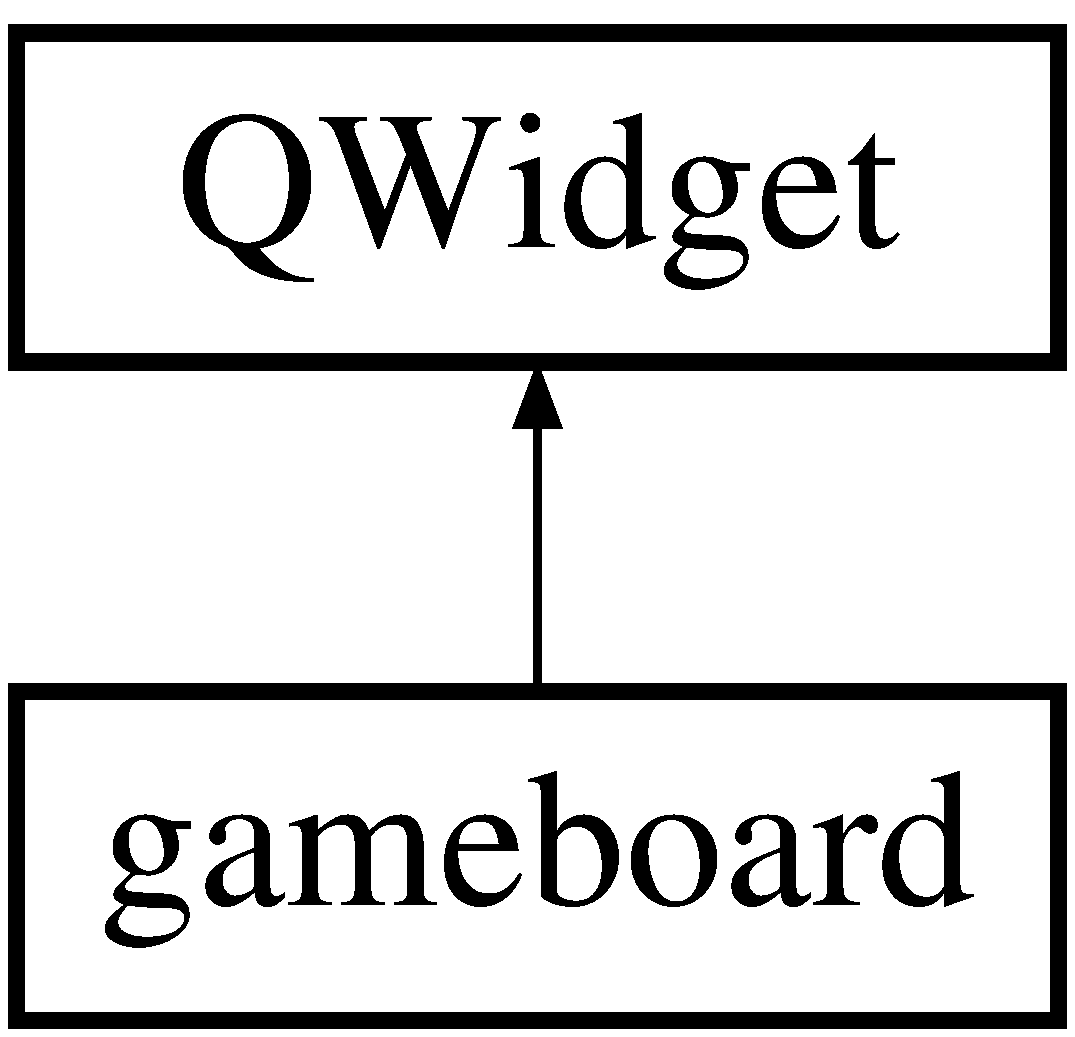
\includegraphics[height=2.000000cm]{classgameboard}
\end{center}
\end{figure}
\subsection*{Public Slots}
\begin{DoxyCompactItemize}
\item 
\hypertarget{classgameboard_a68238b5385a056e5708be1f9918ef07d}{}void \hyperlink{classgameboard_a68238b5385a056e5708be1f9918ef07d}{update\+Enemy} ()\label{classgameboard_a68238b5385a056e5708be1f9918ef07d}

\begin{DoxyCompactList}\small\item\em \hyperlink{classgameboard_a68238b5385a056e5708be1f9918ef07d}{gameboard\+::update\+Enemy} updates the movement of the enemies \end{DoxyCompactList}\item 
\hypertarget{classgameboard_ab509115a3bc5d8c0fa11ced0abd293ed}{}void \hyperlink{classgameboard_ab509115a3bc5d8c0fa11ced0abd293ed}{cat\+Caught} ()\label{classgameboard_ab509115a3bc5d8c0fa11ced0abd293ed}

\begin{DoxyCompactList}\small\item\em \hyperlink{classgameboard_ab509115a3bc5d8c0fa11ced0abd293ed}{gameboard\+::cat\+Caught} if cat is caught by an enemy \end{DoxyCompactList}\item 
\hypertarget{classgameboard_a1c63304bc284a0d8e58934d4370b16ee}{}void \hyperlink{classgameboard_a1c63304bc284a0d8e58934d4370b16ee}{advance\+Level} ()\label{classgameboard_a1c63304bc284a0d8e58934d4370b16ee}

\begin{DoxyCompactList}\small\item\em \hyperlink{classgameboard_a1c63304bc284a0d8e58934d4370b16ee}{gameboard\+::advance\+Level} advances to the next level \end{DoxyCompactList}\end{DoxyCompactItemize}
\subsection*{Signals}
\begin{DoxyCompactItemize}
\item 
\hypertarget{classgameboard_a7bed0743b0684228902113bd840b79ba}{}void {\bfseries game\+\_\+over} ()\label{classgameboard_a7bed0743b0684228902113bd840b79ba}

\end{DoxyCompactItemize}
\subsection*{Public Member Functions}
\begin{DoxyCompactItemize}
\item 
\hyperlink{classgameboard_a45936725b978fc6548d0ad9e62b70d95}{gameboard} (Q\+Widget $\ast$parent=0, Q\+String cat=\char`\"{}charlie\char`\"{}, Q\+String enemy=\char`\"{}mouse\char`\"{})
\item 
\hypertarget{classgameboard_ac10e30eecd45bb004a592f97bd0e398f}{}\hyperlink{classgameboard_ac10e30eecd45bb004a592f97bd0e398f}{$\sim$gameboard} ()\label{classgameboard_ac10e30eecd45bb004a592f97bd0e398f}

\begin{DoxyCompactList}\small\item\em \hyperlink{classgameboard_ac10e30eecd45bb004a592f97bd0e398f}{gameboard\+::$\sim$gameboard} destructor \end{DoxyCompactList}\item 
void \hyperlink{classgameboard_a7c2f3cab761a2d642a0f0fb2b430a21d}{paint\+Event} (Q\+Paint\+Event $\ast$e)
\begin{DoxyCompactList}\small\item\em \hyperlink{classgameboard_a7c2f3cab761a2d642a0f0fb2b430a21d}{gameboard\+::paint\+Event} paints the cat and enemies on board \end{DoxyCompactList}\item 
void \hyperlink{classgameboard_a426162fac3b314115067be644865cdaf}{key\+Press\+Event} (Q\+Key\+Event $\ast$event)
\begin{DoxyCompactList}\small\item\em \hyperlink{classgameboard_a426162fac3b314115067be644865cdaf}{gameboard\+::key\+Press\+Event} defines what happens when the player presses certain keys \end{DoxyCompactList}\item 
void \hyperlink{classgameboard_a62459809a28e3835f62a5311f13e22eb}{show\+Event} (Q\+Show\+Event $\ast$e)
\begin{DoxyCompactList}\small\item\em \hyperlink{classgameboard_a62459809a28e3835f62a5311f13e22eb}{gameboard\+::show\+Event} shows the gameboard event \end{DoxyCompactList}\item 
void \hyperlink{classgameboard_acd4d2cbede5463c4a8c42962766ffe87}{update\+Cat} (int px, int py, int nx, int ny)
\begin{DoxyCompactList}\small\item\em \hyperlink{classgameboard_acd4d2cbede5463c4a8c42962766ffe87}{gameboard\+::update\+Cat} updates the cat position \end{DoxyCompactList}\end{DoxyCompactItemize}


\subsection{Constructor \& Destructor Documentation}
\hypertarget{classgameboard_a45936725b978fc6548d0ad9e62b70d95}{}\index{gameboard@{gameboard}!gameboard@{gameboard}}
\index{gameboard@{gameboard}!gameboard@{gameboard}}
\subsubsection[{gameboard}]{\setlength{\rightskip}{0pt plus 5cm}gameboard\+::gameboard (
\begin{DoxyParamCaption}
\item[{Q\+Widget $\ast$}]{parent = {\ttfamily 0}, }
\item[{Q\+String}]{cat = {\ttfamily \char`\"{}charlie\char`\"{}}, }
\item[{Q\+String}]{enemy = {\ttfamily \char`\"{}mouse\char`\"{}}}
\end{DoxyParamCaption}
)\hspace{0.3cm}{\ttfamily [explicit]}}\label{classgameboard_a45936725b978fc6548d0ad9e62b70d95}
Gameboard constructor that sets the board with the cat and enemy that the player chooses C\+O\+D\+E B\+E\+L\+O\+W S\+E\+T\+S T\+H\+E G\+A\+M\+E\+B\+O\+A\+R\+D

C\+O\+D\+E B\+E\+L\+O\+W C\+O\+M\+B\+I\+N\+E\+S T\+O\+P B\+A\+R W\+I\+T\+H G\+A\+M\+E\+B\+O\+A\+R\+D

C\+O\+D\+E B\+E\+L\+O\+W S\+E\+T\+S T\+H\+E E\+N\+E\+M\+Y N\+U\+M\+B\+E\+R A\+N\+D T\+H\+E\+I\+R R\+A\+N\+D\+O\+M L\+O\+C\+A\+T\+I\+O\+N 

\subsection{Member Function Documentation}
\hypertarget{classgameboard_a426162fac3b314115067be644865cdaf}{}\index{gameboard@{gameboard}!key\+Press\+Event@{key\+Press\+Event}}
\index{key\+Press\+Event@{key\+Press\+Event}!gameboard@{gameboard}}
\subsubsection[{key\+Press\+Event}]{\setlength{\rightskip}{0pt plus 5cm}void gameboard\+::key\+Press\+Event (
\begin{DoxyParamCaption}
\item[{Q\+Key\+Event $\ast$}]{event}
\end{DoxyParamCaption}
)}\label{classgameboard_a426162fac3b314115067be644865cdaf}


\hyperlink{classgameboard_a426162fac3b314115067be644865cdaf}{gameboard\+::key\+Press\+Event} defines what happens when the player presses certain keys 


\begin{DoxyParams}{Parameters}
{\em event} & is the Q\+Key\+Event pointer object \\
\hline
\end{DoxyParams}
\hypertarget{classgameboard_a7c2f3cab761a2d642a0f0fb2b430a21d}{}\index{gameboard@{gameboard}!paint\+Event@{paint\+Event}}
\index{paint\+Event@{paint\+Event}!gameboard@{gameboard}}
\subsubsection[{paint\+Event}]{\setlength{\rightskip}{0pt plus 5cm}void gameboard\+::paint\+Event (
\begin{DoxyParamCaption}
\item[{Q\+Paint\+Event $\ast$}]{e}
\end{DoxyParamCaption}
)}\label{classgameboard_a7c2f3cab761a2d642a0f0fb2b430a21d}


\hyperlink{classgameboard_a7c2f3cab761a2d642a0f0fb2b430a21d}{gameboard\+::paint\+Event} paints the cat and enemies on board 


\begin{DoxyParams}{Parameters}
{\em e} & is the Q\+Paint\+Event pointer object \\
\hline
\end{DoxyParams}
\hypertarget{classgameboard_a62459809a28e3835f62a5311f13e22eb}{}\index{gameboard@{gameboard}!show\+Event@{show\+Event}}
\index{show\+Event@{show\+Event}!gameboard@{gameboard}}
\subsubsection[{show\+Event}]{\setlength{\rightskip}{0pt plus 5cm}void gameboard\+::show\+Event (
\begin{DoxyParamCaption}
\item[{Q\+Show\+Event $\ast$}]{e}
\end{DoxyParamCaption}
)}\label{classgameboard_a62459809a28e3835f62a5311f13e22eb}


\hyperlink{classgameboard_a62459809a28e3835f62a5311f13e22eb}{gameboard\+::show\+Event} shows the gameboard event 


\begin{DoxyParams}{Parameters}
{\em e} & is the Q\+Show\+Event pointer object \\
\hline
\end{DoxyParams}
\hypertarget{classgameboard_acd4d2cbede5463c4a8c42962766ffe87}{}\index{gameboard@{gameboard}!update\+Cat@{update\+Cat}}
\index{update\+Cat@{update\+Cat}!gameboard@{gameboard}}
\subsubsection[{update\+Cat}]{\setlength{\rightskip}{0pt plus 5cm}void gameboard\+::update\+Cat (
\begin{DoxyParamCaption}
\item[{int}]{px, }
\item[{int}]{py, }
\item[{int}]{nx, }
\item[{int}]{ny}
\end{DoxyParamCaption}
)}\label{classgameboard_acd4d2cbede5463c4a8c42962766ffe87}


\hyperlink{classgameboard_acd4d2cbede5463c4a8c42962766ffe87}{gameboard\+::update\+Cat} updates the cat position 


\begin{DoxyParams}{Parameters}
{\em px} & is the current x coordinate of cat \\
\hline
{\em py} & is the current y coordinate of cat \\
\hline
{\em nx} & is new x coordinate of cat \\
\hline
{\em ny} & is new y coordinate of cat \\
\hline
\end{DoxyParams}


The documentation for this class was generated from the following files\+:\begin{DoxyCompactItemize}
\item 
gameboard.\+h\item 
gameboard.\+cpp\end{DoxyCompactItemize}

\hypertarget{classinstruction}{}\section{instruction Class Reference}
\label{classinstruction}\index{instruction@{instruction}}
Inheritance diagram for instruction\+:\begin{figure}[H]
\begin{center}
\leavevmode
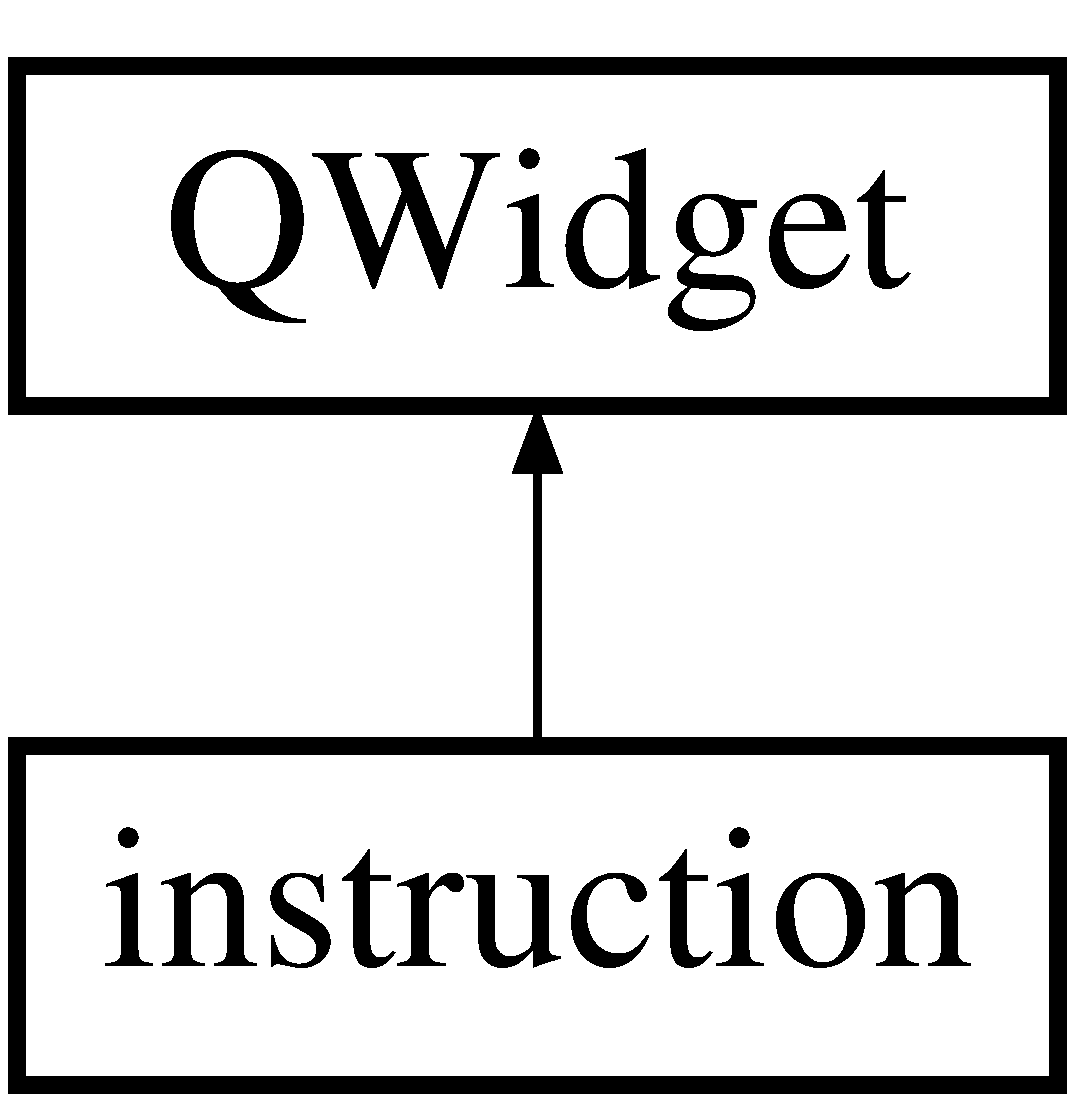
\includegraphics[height=2.000000cm]{classinstruction}
\end{center}
\end{figure}
\subsection*{Public Member Functions}
\begin{DoxyCompactItemize}
\item 
\hypertarget{classinstruction_aef14793380b1853c6d0d1276c40d8f3c}{}{\bfseries instruction} (Q\+Widget $\ast$parent=0)\label{classinstruction_aef14793380b1853c6d0d1276c40d8f3c}

\end{DoxyCompactItemize}


The documentation for this class was generated from the following files\+:\begin{DoxyCompactItemize}
\item 
instruction.\+h\item 
instruction.\+cpp\end{DoxyCompactItemize}

\hypertarget{class_main_window}{}\section{Main\+Window Class Reference}
\label{class_main_window}\index{Main\+Window@{Main\+Window}}
Inheritance diagram for Main\+Window\+:\begin{figure}[H]
\begin{center}
\leavevmode
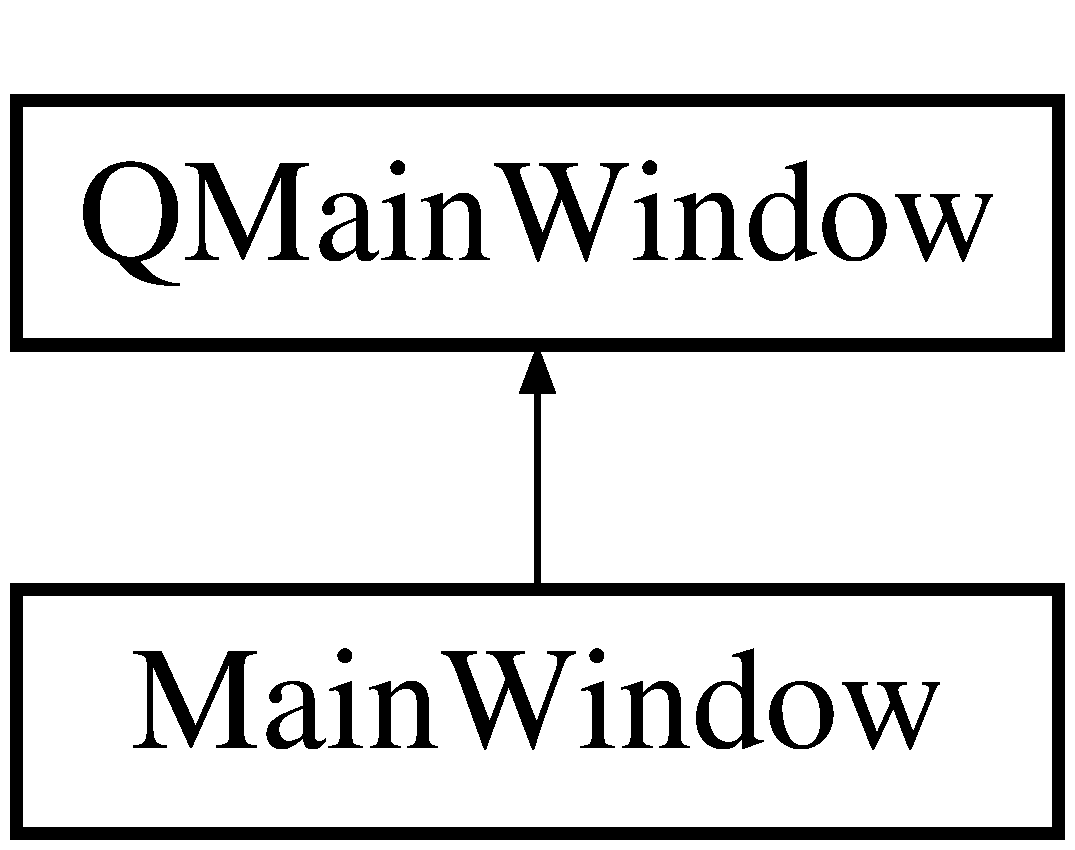
\includegraphics[height=2.000000cm]{class_main_window}
\end{center}
\end{figure}
\subsection*{Public Slots}
\begin{DoxyCompactItemize}
\item 
void \hyperlink{class_main_window_a49fca0e8fb079b547aab74a32bc7baef}{on\+\_\+startbutton\+\_\+clicked} ()
\item 
\hypertarget{class_main_window_a62d37a81c0f9509fbe7ce023563e2f55}{}void \hyperlink{class_main_window_a62d37a81c0f9509fbe7ce023563e2f55}{charlie\+\_\+clicked} ()\label{class_main_window_a62d37a81c0f9509fbe7ce023563e2f55}

\begin{DoxyCompactList}\small\item\em \hyperlink{class_main_window_a62d37a81c0f9509fbe7ce023563e2f55}{Main\+Window\+::charlie\+\_\+clicked} check if player picked charlie. \end{DoxyCompactList}\item 
\hypertarget{class_main_window_af7fed86d97e632ec10688deaaf40a9bd}{}void \hyperlink{class_main_window_af7fed86d97e632ec10688deaaf40a9bd}{grumpy\+\_\+clicked} ()\label{class_main_window_af7fed86d97e632ec10688deaaf40a9bd}

\begin{DoxyCompactList}\small\item\em \hyperlink{class_main_window_af7fed86d97e632ec10688deaaf40a9bd}{Main\+Window\+::grumpy\+\_\+clicked} check if player picked grumpy cat. \end{DoxyCompactList}\item 
\hypertarget{class_main_window_abf315b2e51762568c3613df5174f2edf}{}void \hyperlink{class_main_window_abf315b2e51762568c3613df5174f2edf}{nyancat\+\_\+clicked} ()\label{class_main_window_abf315b2e51762568c3613df5174f2edf}

\begin{DoxyCompactList}\small\item\em \hyperlink{class_main_window_abf315b2e51762568c3613df5174f2edf}{Main\+Window\+::nyancat\+\_\+clicked} check if player picked nyancat. \end{DoxyCompactList}\item 
\hypertarget{class_main_window_ae18d7434c70c6d778a308754e2f45544}{}void \hyperlink{class_main_window_ae18d7434c70c6d778a308754e2f45544}{mouse\+\_\+clicked} ()\label{class_main_window_ae18d7434c70c6d778a308754e2f45544}

\begin{DoxyCompactList}\small\item\em \hyperlink{class_main_window_ae18d7434c70c6d778a308754e2f45544}{Main\+Window\+::mouse\+\_\+clicked} check if player picked mouse dog as enemy. \end{DoxyCompactList}\item 
\hypertarget{class_main_window_a6fda2b6088de157a1e17c549dfa2b535}{}void \hyperlink{class_main_window_a6fda2b6088de157a1e17c549dfa2b535}{dog\+\_\+clicked} ()\label{class_main_window_a6fda2b6088de157a1e17c549dfa2b535}

\begin{DoxyCompactList}\small\item\em \hyperlink{class_main_window_a6fda2b6088de157a1e17c549dfa2b535}{Main\+Window\+::dog\+\_\+clicked} check if player picked dog as enemy. \end{DoxyCompactList}\item 
\hypertarget{class_main_window_ac77fd9a7046d941d9911f8ef276acc92}{}void \hyperlink{class_main_window_ac77fd9a7046d941d9911f8ef276acc92}{human\+\_\+clicked} ()\label{class_main_window_ac77fd9a7046d941d9911f8ef276acc92}

\begin{DoxyCompactList}\small\item\em \hyperlink{class_main_window_ac77fd9a7046d941d9911f8ef276acc92}{Main\+Window\+::human\+\_\+clicked} check if player picked human as enemy. \end{DoxyCompactList}\item 
\hypertarget{class_main_window_ad095804e948ea80ebaa1311858700ded}{}void \hyperlink{class_main_window_ad095804e948ea80ebaa1311858700ded}{game\+\_\+over} ()\label{class_main_window_ad095804e948ea80ebaa1311858700ded}

\begin{DoxyCompactList}\small\item\em \hyperlink{class_main_window_ad095804e948ea80ebaa1311858700ded}{Main\+Window\+::game\+\_\+over} changes window screen when game is over. \end{DoxyCompactList}\end{DoxyCompactItemize}
\subsection*{Public Member Functions}
\begin{DoxyCompactItemize}
\item 
\hyperlink{class_main_window_a8b244be8b7b7db1b08de2a2acb9409db}{Main\+Window} (Q\+Widget $\ast$parent=0)
\item 
\hyperlink{class_main_window_ae98d00a93bc118200eeef9f9bba1dba7}{$\sim$\+Main\+Window} ()
\end{DoxyCompactItemize}


\subsection{Constructor \& Destructor Documentation}
\hypertarget{class_main_window_a8b244be8b7b7db1b08de2a2acb9409db}{}\index{Main\+Window@{Main\+Window}!Main\+Window@{Main\+Window}}
\index{Main\+Window@{Main\+Window}!Main\+Window@{Main\+Window}}
\subsubsection[{Main\+Window}]{\setlength{\rightskip}{0pt plus 5cm}Main\+Window\+::\+Main\+Window (
\begin{DoxyParamCaption}
\item[{Q\+Widget $\ast$}]{parent = {\ttfamily 0}}
\end{DoxyParamCaption}
)\hspace{0.3cm}{\ttfamily [explicit]}}\label{class_main_window_a8b244be8b7b7db1b08de2a2acb9409db}
Mainwindow constructor \hypertarget{class_main_window_ae98d00a93bc118200eeef9f9bba1dba7}{}\index{Main\+Window@{Main\+Window}!````~Main\+Window@{$\sim$\+Main\+Window}}
\index{````~Main\+Window@{$\sim$\+Main\+Window}!Main\+Window@{Main\+Window}}
\subsubsection[{$\sim$\+Main\+Window}]{\setlength{\rightskip}{0pt plus 5cm}Main\+Window\+::$\sim$\+Main\+Window (
\begin{DoxyParamCaption}
{}
\end{DoxyParamCaption}
)}\label{class_main_window_ae98d00a93bc118200eeef9f9bba1dba7}
Mainwindow destructor 

\subsection{Member Function Documentation}
\hypertarget{class_main_window_a49fca0e8fb079b547aab74a32bc7baef}{}\index{Main\+Window@{Main\+Window}!on\+\_\+startbutton\+\_\+clicked@{on\+\_\+startbutton\+\_\+clicked}}
\index{on\+\_\+startbutton\+\_\+clicked@{on\+\_\+startbutton\+\_\+clicked}!Main\+Window@{Main\+Window}}
\subsubsection[{on\+\_\+startbutton\+\_\+clicked}]{\setlength{\rightskip}{0pt plus 5cm}void Main\+Window\+::on\+\_\+startbutton\+\_\+clicked (
\begin{DoxyParamCaption}
{}
\end{DoxyParamCaption}
)\hspace{0.3cm}{\ttfamily [slot]}}\label{class_main_window_a49fca0e8fb079b547aab74a32bc7baef}
The pushbutton start changes mainwindow to gameboard 

The documentation for this class was generated from the following files\+:\begin{DoxyCompactItemize}
\item 
mainwindow.\+h\item 
mainwindow.\+cpp\end{DoxyCompactItemize}

%--- End generated contents ---

% Index
\backmatter
\newpage
\phantomsection
\clearemptydoublepage
\addcontentsline{toc}{chapter}{Index}
\printindex

\end{document}
